\chapter{Elements of fracture mechanics and DIC method}
\label{Chapter2}

\section{Introduction}

Fracture mechanics aim is to characterise the cracking behaviour of diverse and complex structures using parameters that can be quantified in an engineering sense, including the stress field, crack size and cracking resistance of the material. The first theoretical developments in the analysis of displacement, strain and stress fields in the vicinity of a crack were undertaken around 1940. Since then, the development of fracture mechanics has extended to materially and geometrically nonlinear problems, mixed mode crack bifurcation problems and more recently to composites, numerical solution techniques and the state of the art in the design of various complex structures. The objective of applied fracture mechanics is to characterize the cracking behavior of structures using quantifiable parameters in the engineering sense, including stress, crack size, and material resistance to cracking.

In this chapter, a look is taken at fracture mechanics with applications to wood material. Essential notions will be reminded in order to understand the mechanics of linear fracture. First, we will look at different types of specimens used for similar studies, and then at the mechanical orthotropic fields. The second part of the chapter is devoted to the explanation of the DIC method, in particular its operation and its use.

\section{Test pieces used in fracture mechanics}

There are three ways of applying a force to allow a crack to propagate as shown figure \ref{fig:fig14}. Mode I is a tensile stress normal to the crack plane, mode II is a shear stress acting parallel to the crack plane and perpendicular to the crack front. Mode III is a shear stress acting parallel to the crack plane and parallel to the crack front. In general, a crack propagates in a material under a combination of stresses in all three modes. These modes can be presenting by the energy release rate (G) linked to crack length. It is called R-curve and has three characterized propagation crack zones. A first increasing phase of instability to initiate the cracking process. A second phase, which corresponds to a stabilised propagation range during which only viscoelastic effects (creep) will participate in the advance of the crack front and a last phase which symbolises the ruin of the material.

\graphicspath{{Images/}}
\begin{figure}[htp]
	\centering
	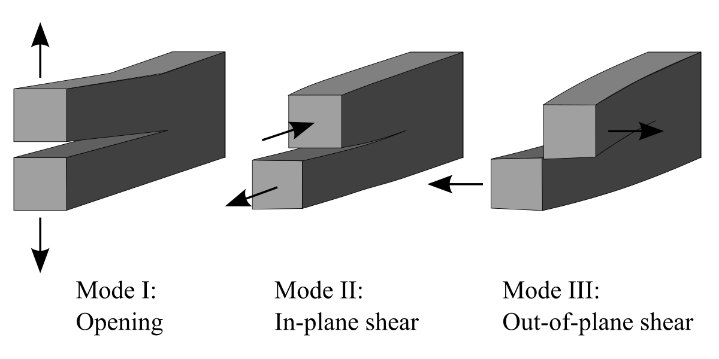
\includegraphics[width=10cm]{fig14}
	\caption{Illustration of the three modes of rupture}
	\label{fig:fig14}
\end{figure}

Moreover, the cracking failure mechanism can occur in two types of cracking: 

\begin{itemize}
	\item Abrupt cracking: for solids, or for very high strength materials, the working stresses are very high, and considerable potential energy is thus created; the presence of small cracks can then lead to abrupt failure which is often not accompanied by macroscopic plastic deformations due to the very low ductility. 
	\item Successive cracking: this is a succession of mechanisms (brittle - ductile) which, under repeated stresses, leads to successive cracking or fatigue failure. The factors that influence the cracking behaviour of materials are of two kinds: metallurgical and mechanical. The mechanical factors relate to the state of displacements, strains and stresses, as well as environmental conditions such as temperature or relative humidity. It is easier to observe because it takes more time to involve samples destruction than a unique and sudden crack. With a material like wood, successive cracks rupture are expected.
\end{itemize}

In order to realize these different modes of rupture, we need specimens that meet certain criteria such as geometry. Indeed, some specimens were designed to solve problems for mode I while others for mode II or mixed mode. There are therefore several types of test specimens:

\smallskip

\textbf{DCB test piece}

The double cantilever beam (DCB) specimen was developed for testing in the crack opening mode (Mode I). Its design allows to obtain a stress intensity factor that decreases when the crack propagates. However, it also allows the determination of the toughness and the critical energy restitution rate in mode I and mode II. Indeed, in the document of [YOS 2008] Mode I and Mode II fracture toughness were measured of compressed spruce by a double cantilever beam (DCB) test and a three-point bend end notched flexure (3ENF) test figure \ref{fig:fig15}.

\graphicspath{{Images/}}
\begin{figure}[htp]
	\centering
	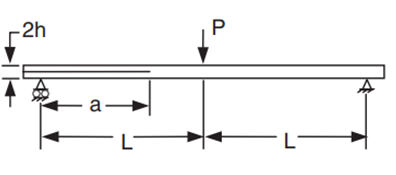
\includegraphics[width=5cm]{fig15}
	\caption{Schematic representation of 3ENF test with DCB test piece. [DAV 2005]}
	\label{fig:fig15}
\end{figure}

\smallskip

\textbf{Double Cantilever Beam specimen with variable inertia}

The classical DCB specimen had an instability from the beginning of the crack initiation. This is why Dubois [DUB 2002] proposed a variable inertia DCB specimen with crack stability. The DCB specimen with variable inertia figure \ref{fig:fig16} was designed to ensure stabilised propagation in Mode I. Thus, after the crack initiation zone, a decrease in the rate of elastic energy restitution G is observed over a given propagation range. During this phase, only viscoelastic effects will participate in the progression of the crack front when the specimen is loaded in creep. The viscoelastic characteristics will thus be clearly decoupled from the cracking parameters. 

\graphicspath{{Images/}}
\begin{figure}[htp]
	\centering
	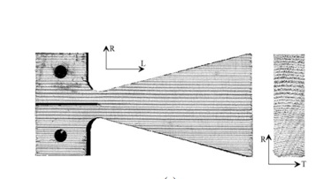
\includegraphics[width=5cm]{fig16}
	\caption{DCB specimen with variable inertia [DUB 2002]}
	\label{fig:fig16}
\end{figure}

\smallskip

\textbf{Compact Tension Shear specimen}

The Compact Tension Shear (CTS) specimen figure \ref{fig:fig17} is designed to evaluate all mixed modes in different materials. It was developed for mixed loads in isotropic materials. Two steel arms are pierced with holes where symmetrical forces P oriented by angles $\beta$ of mixtures are applied. On both specimens, the crack remains oriented in the direction of high orthotropy.

\graphicspath{{Images/}}
\begin{figure}[htp]
	\centering
	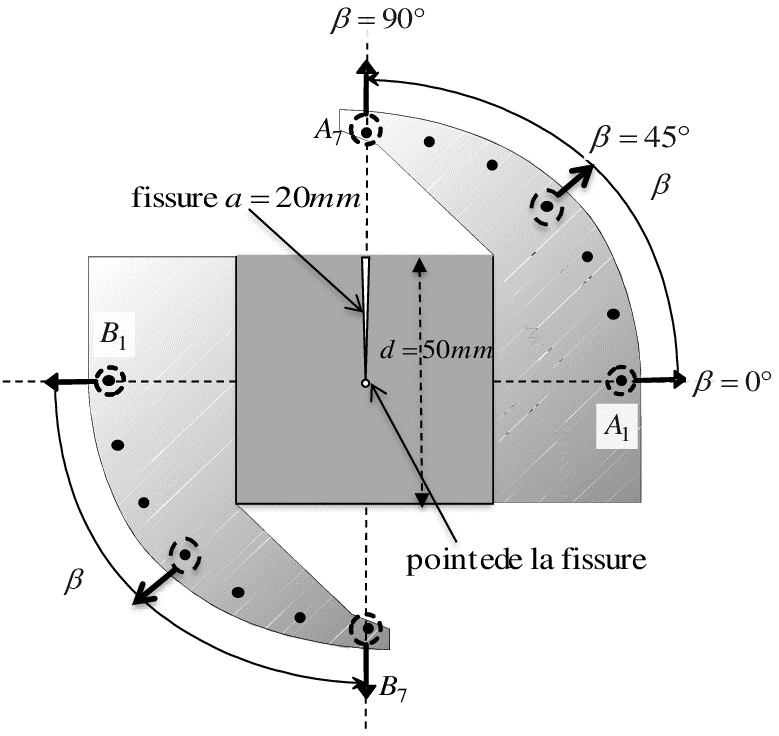
\includegraphics[width=5cm]{fig17}
	\caption{Compact Tension Shear (CTS) specimen}
	\label{fig:fig17}
\end{figure}


\textbf{Mixed Mode Crack Growth specimen}

The design of the Mixed Mode Crack Growth (MMCG) specimen figure \ref{fig:fig18} was based on a combination of the two geometric solutions described above. The original DCB specimen was modified by adding a lower heel to secure the mixed mode loading device. The upper heel was slightly inclined to ensure stiffness in the vicinity of the two connection fillets. The body of the specimen has increasing inertia towards the crack tip to ensure a stable rate of energy restitution. Four symmetrically arranged PVC arms are attached to the wooden specimen. Boreholes are provided to allow for loads with a variable $\beta$-mixing rate identical to that of the CTS specimen. This test piece allows for a given propagation range, in mode 1, mode 2 and in mixed mode, a stability or even a considerable decrease of the energy restitution rate[MOU 2008].

\graphicspath{{Images/}}
\begin{figure}[htp]
	\centering
	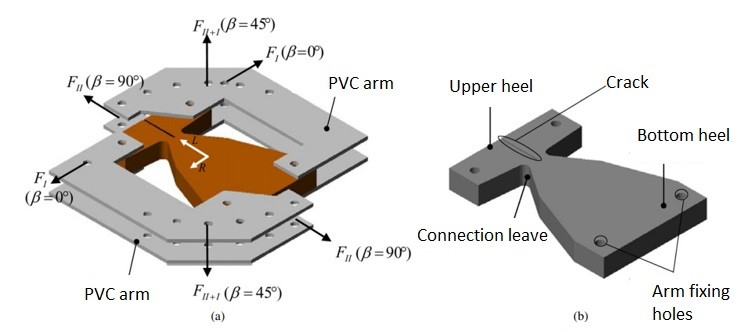
\includegraphics[width=10cm]{fig18}
	\caption{2MCG test piece [MOU 2008]}
	\label{fig:fig18}
\end{figure}

\section{Stress and strain fields}

It is important to notice that different zones are studied. In fracture mechanics, three successive zones visible figure \ref{fig:fig19} can be distinguished schematically in a cracked medium [MOU 2020]:

\begin{itemize}
	\item The development zone or zone 1: the zone closest to the crack tip. In this part the material is very damaged, which makes its mechanical evaluation rather complex. The size of this zone determines the type of cracking that will occur. Indeed, if the size of the zone is large, ductile cracking will be observed. On the other hand, if it is small, brittle cracking will be observed.
	\item The singular zone or zone 2: this covers the entire development zone. In this zone, the displacement, strain and stress fields are continuous and have a formulation that is independent of the distant geometry of the structure. The material has a linear viscoelastic behaviour. Its boundary with zone 1 is assumed to be continuous in stress and displacement.
	\item The far zone or zone 3: this is the zone furthest from the crack. It connects the singular zone with the loading and displacement boundary conditions.
\end{itemize}

\graphicspath{{Images/}}
\begin{figure}[htp]
	\centering
	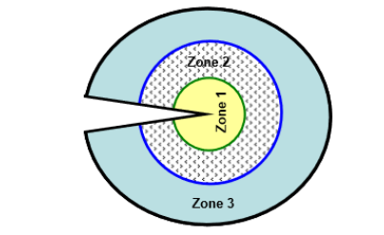
\includegraphics[width=10cm]{fig19}
	\caption{Cracking zone [MOU 2020]}
	\label{fig:fig19}
\end{figure}

For a linear elastic material, the stress field at a point M in the vicinity of the crack can be expressed simply as a function of the stress intensity factor $K_{I,II,III}$ and the polar coordinates ( r, $\theta$). The dimensionless functions $f_{ij}$  and  $g_{ij}$ depend on the mode of loading. The intensity factor is independent of the point M. Moreover, in the vicinity of the crack tip the value of r is very small, and tends to 0. Thus the stress field is expressed :

\begin{equation}
	\sigma_{i,j} = \frac{K_{\beta}}{\sqrt{2*\pi*r}}*f_{i,j}(\theta)
	\label{eq:1}
\end{equation}

The coefficient $K_\beta$ in the equation \ref{1} is the stress intensity factor (mode I and mode II) and is independent of the point M, Figure \ref{fig:fig20}.

\graphicspath{{Images/}}
\begin{figure}[htp]
	\centering
	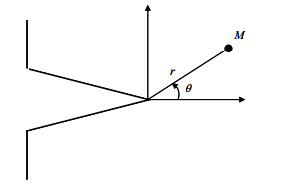
\includegraphics[width=10cm]{fig20}
	\caption{Crack tip scoring}
	\label{fig:fig20}
\end{figure}

We have seen that there are three ways of applying a force, to a specimen, to allow a crack to propagate. These modes define the expression of the mechanical field in zone 2 for orthotropic material. They are defined and expressed as follows and are illustrated in Figure \ref{fig:fig14}[ODO 2018]:

\textbf{Mechanical fields in the singular zone for mode 1}

\begin{equation}
	\sigma_{1,1} = \frac{K_{1}}{\sqrt{2 \pi r}} \cos{\frac{\theta}{2}}  \left( 1-\sin{\frac{\theta}{2}} \sin{\frac{3 \theta}{2}} \right)
\end{equation}

\begin{equation}
	\sigma_{2,2} = \frac{K_{1}}{\sqrt{2 \pi*r}} \cos{\frac{\theta}{2}}  \left( 1+\sin{\frac{\theta}{2}} \sin{\frac{3 \theta}{2}} \right)
\end{equation}

\begin{equation}
	\sigma_{1,2} = \frac{K_{1}}{\sqrt{2 \pi r}} \cos{\frac{\theta}{2}}  \sin{\frac{\theta}{2}} \cos{\frac{3 \theta}{2}}
\end{equation}

The displacement field for the mode 1 loading is written as follows:

\begin{equation}
	u_{1} = \frac{K_{1}}{4 \pi}*\sqrt{\frac{r}{2 \pi}} \left((2 \chi-1) \sin{\frac{\theta}{2}}-\sin{\frac{3 \theta}{2}}\right)
\end{equation}

\begin{equation}
	u_{2} = \frac{K_{1}}{4 \pi} \sqrt{\frac{r}{2*\pi}} \left((2 \chi+1) \sin{\frac{\theta}{2}}-\sin{\frac{3 \theta}{2}}\right)
\end{equation}

With : 

$K_1$  the mode 1 stress intensity factor

$\mu=\frac{E}{2 (1+\nu)}$ , the shear coefficient of Lame

$\nu=\frac{\lambda}{2 (\lambda+\mu)}$ , the shear coefficient of Poisson

$E=\frac{\mu (3 \lambda+2 \mu)}{\lambda+\mu}$, the Young modulus

$\lambda=\frac{\nu E}{(1-2 \nu)(1+\nu)}$ , the Lame’s Coefficients

The term $\chi$ is a constant defined as follows:\ $\chi=3-4\nu$ for plane deformations and \ $\chi=\frac{3-\nu}{1-\nu}$  for plane stresses.

r and $\theta$ polar coordinates of point M centred on the crack tip, Figure 11

\smallskip

\textbf{Mechanical fields in the singular zone for mode 2}

\begin{equation}
	\sigma_{1,1} = \frac{-K_{2}}{\sqrt{2 \pi r}} \sin{\frac{\theta}{2}}  \left( 2+\cos{\frac{\theta}{2}} \cos{\frac{3 \theta}{2}} \right)
\end{equation}

\begin{equation}
	\sigma_{2,2} = \frac{K_{2}}{\sqrt{2 \pi r}} \cos{\frac{\theta}{2}}  \sin{\frac{\theta}{2}} \cos{\frac{3 \theta}{2}}
\end{equation}

\begin{equation}
	\sigma_{1,2} = \frac{K_{2}}{\sqrt{2 \pi r}} \cos{\frac{\theta}{2}}  \left( 1-\sin{\frac{\theta}{2}} \sin{\frac{3 \theta}{2}} \right)
\end{equation}

The displacement field for the mode 2 loading is written as follows:

\begin{equation}
	u_{1} = \frac{-K_{2}}{4 \pi} \sqrt{\frac{r}{2 \pi}} \left((2 \chi+3) \sin{\frac{\theta}{2}}+\sin{\frac{3 \theta}{2}}\right)
\end{equation}

\begin{equation}
	u_{2} = \frac{K_{2}}{4 \pi} \sqrt{\frac{r}{2 \pi}} \left((2 \chi+3) \cos{\frac{\theta}{2}}+\cos{\frac{3 \theta}{2}}\right)
\end{equation}

With : $K_2$  the mode 2 stress intensity factor

\smallskip

\textbf{Mechanical fields in the singular zone for mode 3}

\begin{equation}
	\sigma_{1,3} = \frac{-K_{3}}{\sqrt{2 \pi r}} \sin{\frac{\theta}{2}}
\end{equation}

\begin{equation}
	\sigma_{2,3} = \frac{K_{3}}{\sqrt{2 \pi r}} \cos{\frac{\theta}{2}}
\end{equation}

The displacement field for the mode 3 loading is written as follows:

\begin{equation}
	u_{3} = \frac{-2 K_{3}}{\mu} \sqrt{\frac{r}{2 \pi}} \sin{\frac{\theta}{2}}
\end{equation}

With : $K_3$  the mode 3 stress intensity factor

\section{Method of the complacency}

In this part we give and define the different terms of the imposed displacement complacency formula. This formula will be used in the next chapters to calculate the energy restitution rate. It is defined by the ratio of two parameters: the variation of energy per unit area cracked and the crack propagation in a linear elastic material. The crack propagation will occur when the energy G reaches a critical value noted Gc. This value Gc is a measure of the toughness of the material. Let us now define the mathematical expression of G. First, let us consider a material with a crack of length a and thickness b. A crack propagation $\Delta$a will be accompanied by the following energy variations:

\begin{equation}
	\Delta W_{ext}=\Delta W_{elast}+\Delta U
\end{equation}

With:

$\Delta W_{ext}$ the applied energy change (due to external forces).

$\Delta W_{elast}$ the change in dissipated energy ;

$\Delta$U the energy expended during crack propagation over the length $\Delta$a.

The energy G reported to the unit area will be :

\begin{equation}
	G = \lim_{\Delta \to 0}= \frac{\Delta U}{\Delta A}= \frac{\partial U}{\partial A}
\end{equation}

Where $\Delta A=b\Delta a$  is the cracked area during crack propagation. b is usually equal to 1 because a unit thickness is often considered. Therefore, the energy per unit thickness will be of the form :

\begin{equation}
	G = \lim_{\Delta \to 0}= \frac{\Delta U}{\Delta a}= \frac{\partial U}{\partial a}
\end{equation}

In order to understand the meaning of the energy restitution rate, we will consider, from an initial configuration, the propagation (in a specimen of unit thickness) in the following two classical cases (Figure 18):

\begin{itemize}
	\item propagation with imposed displacement d ; 
	\item propagation with imposed force F.
\end{itemize}

\begin{figure}[htp]
	\centering
	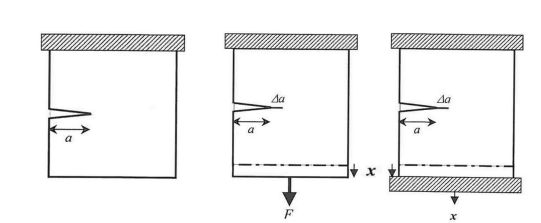
\includegraphics[width=10cm]{fig21}
	\caption{Stable propagation with imposed force or imposed displacement [ZEG 2003].}
	\label{fig:fig21}
\end{figure}

In our work we will limit ourselves to the case of propagation with imposed displacement. In this case if $\Delta x=0$ (with $\Delta x$ variation of the crack), the external energy variation will be zero, we then deduce the elastic energy :

$W_{elast}=\frac{Fx}{2}$

By introducing the complacency by the relation :

$C=\frac{x}{F}$

We deduce :

$W_{elast}=\frac{CF^2}{2}=\frac{x^2}{2C}$

$\Delta W_{elast}=\frac{\partial W_{elast}}{\partial a}\Delta a=\frac{\partial W_{elast}}{\partial a}\ \frac{\partial C}{\partial a}\Delta a=\frac{-x^2}{2C^2}\ \frac{\partial C}{\partial a}\Delta a$

And because we have:

$\Delta W_{ext}=0=\Delta W_{elast}+\Delta U\leftrightarrow \Delta U =-\Delta W_{elast}$

Then we have:

$\Delta U=\frac{x^2}{2C^2}\ \frac{\partial C}{\partial a}\Delta a$

Which enables to obtain:

\begin{equation}
	G=\frac{x^2}{2C^2}\ \frac{\partial C}{\partial a}=\frac{F^2}{2}\ \frac{\partial C}{\partial a}
	\label{2}
\end{equation}

The relationship in equation \ref{2} is related to the unit thickness. In the case where $b\neq1$
we obtain:

\begin{equation}
	G_c=\frac{{F_{ci}}^2}{2b}\ \frac{\partial C}{\partial a}
\end{equation}

With:

$G_c$ the value of energy release rate (in $J/m^2$)

$F_{ci}$ the critical force which involves the crack (in N)

b the thickness of the specimen (in mm)

$F_{ci}$ the complacency evolution (in ${Pa}^{-1}$)

$F_{ci}$ the crack length evolution (in mm)



\section{Software and DIC method}

\subsection{Dic method}

Digital image correlation (DIC) was developed in 1983. It is a 2D or 3D optical method that measures displacements between two images. It is increasingly used in materials science to determine strain fields, detect cracks or to provide displacement fields for material property identification procedures. It is a non-contact optical method of measuring kinematic fields, based on the comparison of the signal amplitude. It relies on the grey levels of the images. The particles are optically tracked using computer algorithms to determine displacements and velocities. Rather than tracking moving particles in a fluid, DIC tracks changes in the relative position of the high contrast surface finish. It works by comparing two images, one reference and one deformed, taken during loading. Thus it must detect a pattern in the reference image and compare it to the pattern in the other images [MAM 2018]. The DIC formulation relies on the conservation of grey levels between the two instants at which the reference images S0 and the current images St are recorded. In other words, this principle is based on the comparison between a reference image and a distorted image. Each image is composed of pixels, and each pixel as a function of the light flux returns information. For 8-bit images, for example, a pixel can have a value between 0 for black and 255 for white. Each image is therefore stored in the form of a two-dimensional matrix whose cells correspond to a value. These matrices are the image correlation data. DIC compares these matrices and deduces the surface displacement field. To do this, during the analysis, the algorithm in place searches for a correlation zone, predefined in the reference image, in that of the image in the deformed state figure \ref{fig:fig22}.

\graphicspath{{Images/}}
\begin{figure}[htp]
	\centering
	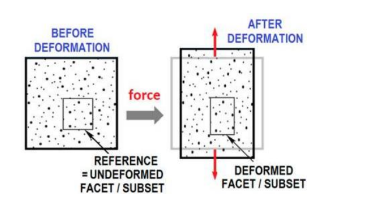
\includegraphics[width=10cm]{fig22}
	\caption{Example of captured images obtained by a camera for image analysis.}
	\label{fig:fig22}
\end{figure}

The system consists of a digital camera and specialised computer software like MatchID. The camera is used to capture consecutive images of the surface of the sample under test before and during the deformation test. The digital images thus determined, which correspond to a series of photographs, are analysed by the DIC software. Displacement maps of the sample on the surface are created. The stress fields can be evaluated from the strain fields. The formula used to obtain the displacement field is shown below equation \ref{3}:

\begin{equation}
	u^k=\left[{u_z^k\atop u_y^k}\right]=\sum_{i=1}^{N}\left\{\left[{{\ \ f}_i\left(k,\Phi_k\right)\ \ {\ \ g}_i\left(k,\Phi_k\right)\atop{\ \ l}_i\left(k,\Phi_k\right)\ \ {\ \ m}_i\left(k,\Phi_k\right)}\right]\times\left[{A_1^i\atop A_2^i}\right] \times r_k^{i/2}\right\}+\left[{T_x\atop T_y}\right]+R\times\left[{y_k\atop x_k}\right] 
	\label{3}
\end{equation}

With the polar functions $f_i$, $g_i$, $l_i$, $m_i$, k depends on the material because of the Poisson's ratio term which determines k. The T terms are correction factors for rigid body movements.

If this method is used on wood, it is important to note that the 2D orthotropic elastic material model has five engineering constants as input parameters, to be entered into the image analysis system. Although it depends on the software used, it is important to know these inputs. Firstly, the Young's modulus in the longitudinal direction must be entered, $E_L=E_1$, the transverse Young's modulus $E_{trans}=E_R=E_T=E_2$. Then the shear modulus $G_{LR}=G_{LT}=G_{12}$, if the shear mode is studied. Therefore, the Poisson's ratio $\nu$ has to be introduced in the software. This coefficient can change depending on the surface under study, in or out of the plane. The initial crack length is introduced into the model. The description of the damage is presented by three main inputs, although it may change depending on the software. If we are in mode I damage, it is described by the damage initiation stress $\sigma_{ini}$, but also by the failure stress $\delta_{fl}$, and the shape coefficient of the exponential function $\alpha_l$.

\subsection{Characteristic of the Wood used}

In this section, the values of the mechanical characteristics (moduli of elasticity, compliances and shear coefficients) are given. As no characterization tests were carried out in this study, the data from the literature are used here, following the document created by Guitard[GUI 1987]. These values which are the shearing $G_{ij}$ and longitudinal modulus $E_i$ , the Poisson’s coefficient $\nu_{ij}$ and $\rho$ change for each species. Moreover, these values can evolve due to temperature and relative humidity. By knowing the temperature, the relative humidity and the volume weight of a specimen, it is possible to obtain the characteristics wanted. Table \ref{fig:fig28} and \ref{fig:fig29} give us the characteristics for the Pinus Sp Pine at 9.7$\%$ humidity:

\graphicspath{{Images/}}
\begin{table}[htp]
	\centering
	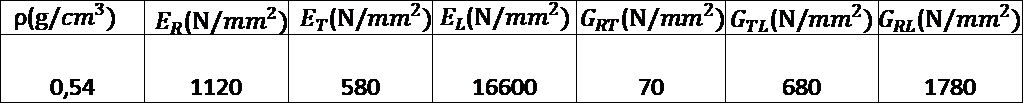
\includegraphics[width=10cm]{fig28}
	\caption{Characteristic of the Pinus Sp Pine}
	\label{fig:fig28}
\end{table}

\graphicspath{{Images/}}
\begin{table}[htp]
	\centering
	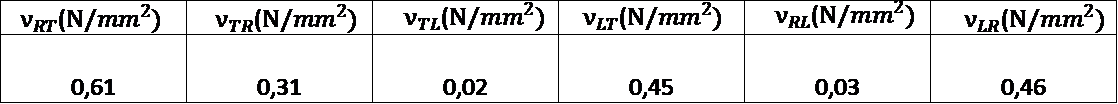
\includegraphics[width=10cm]{fig29}
	\caption{Characteristic of the Pinus Sp Pine}
	\label{fig:fig29}
\end{table}

\subsection{Preparation of the DIC method}

Before starting the measurements with the DIC method, it is important to define some parameters. In our case, the quantity of interest is the crack length a as a function of the applied force F. It is also important to define the zone of interest (ZOI). It is the portion of the image corresponding to the zone-of-interest of the test piece.. The field of view ( FOV), the position envelope for hardware and if the test is a 2D-DIC or a stereo DIC are parameters to take into account. In our case, a 2D-DIC is suitable because the test piece is assumed to be planar and perpendicular to the camera optical axis. The camera and lens have to be well selected in order to obtain the desired FOV and spatial resolution for example. With a pre-determined aperture of the lens, it’s important to select lighting and an exposure time to have sufficient contrast between the white and black regions of the DIC pattern. The contrast should be uniform over the entire ZOI of the image and constant in time. The DIC pattern is one important parameter. All the specimens are painted to obtain a speckle pattern suitable for image correlation. A thin layer of white paint is firstly added using a mate spray, followed by a diffuse distribution of black paint to create a unique local pattern across the ZOI at the crack tip. Estimate the spatial gradients which means determine such as the subset size and the step size. This will determine the required spatial resolution of the DIC system. It’s also necessary to determine the acceptable noise floor and the frame rate. The DIC images need to be synchronized to the force applied by the press. To finish, the calibration must be done. The goal of calibration of a 2D-DIC system is to establish the image scale, i.e. the number of pixels in the image that corresponds to a certain physical distance on the test piece, and to correct for lens distortions.

\subsection{MatchID}

Once the tests are completed, the data is saved on a hard disk for processing. It is possible to process the images with different software. Mambili used Ncorr and matlab while Stanislas Malfait used MatchID and Python. This image processing will allow to obtain the maps of deformations and displacements. For this work will be used matchid and python.

With the MatchID software several steps are necessary:

\begin{itemize}
	\item Choose a reference image that corresponds to the first image of the test 
	\item Select multiple deformed images
	\item Define the zone of interest (ZOI) in which the crack propagates
	\item Define the analysis parameters of the ZOI
	\item Start the DIC analysis
	\item Exploit the results
\end{itemize}

Despite the progress and increasing use of DIC, the technique is still not standardized. It is emphasized that extrinsic and intrinsic DIC setup parameters, such as subset size, subset step, strain gauge window, shape functions, or correlation criterion, can have a considerable influence on the calculated strain fields, producing spatial resolution and resolution values that can differ by at least an order of magnitude. This paragraph will try to explain some of them. 
The correlation criterion defines the matching criterion that will be adopted in order to determine the optimum corresponding point. [MAL 2021]  used the criterion ZNSSD. It is a least-square-based correlation criterion which is less sensitive to both image contrast reduction and light intensity shifting between images. There are 5 subset shape function which allow or not the subset certain constraints as the fact of translating, deforming, to shear etc.. Depending on the local deformation or strain gradients of the problem under analysis, affine, irregular and quadratic shape functions can be selected by the user in the DIC method [PER 2018]. The subset size is the length of the subset in the reference image and it must contain at least 3 speckles. As an indication, larger subsets improve resolution but decrease spatial resolution. This means that in a conventional mechanical tensile test with a uniform, uniaxial stress state in the central region of the specimen, large subsets can be selected to improve the accuracy of the measurements. The step size is the spacing of pixel grid points at which the subset displacements are calculated. It controls the density of points at which DIC data is computed and, to some extent, influences the spatial resolution of the measurements. Typically, a step size of one-third to one-half of the subset size is recommended, so that neighboring subsets partially overlap, though this value can vary widely depending on specific applications. Additionally, a small step size may be required to capture the peak position of a Quantity Of Interest (QOI) (without interpolation) if it varies quickly across the ZOI and if the QOI varies slowly across the ZOI, then a large step size can be used. The strain window is the local region of the ZOI of the image, containing a finite number of data points, that is used to calculate strain. Parameters such as the subset step and the strain window will define a strain spatial resolution and virtual strain gauge (VSG). VSG is the local region of the image that affects the strain value at a specific location. The three dominant variables that affect the VSG size are the subset size, step size, and strain window. If the maximum strain amplitude converges with further decreases of the VSG, then the actual maximum strain amplitude has been captured. Any VSG that is larger than the largest VSG that results in the converged actual maximum strain amplitude will underestimate the actual strain amplitude, and introduce bias into the measured strain results. If the smallest VSG allowed by the software is not sufficient, the test could be repeated with a smaller FOV. The final decision as to which size VSG to use is a matter of judgment. If capturing the highest strain gradient is essential for DIC analysis, a small VSG may be the best choice, even if noise is important. Conversely, if there are no high strain gradients it may be preferable to choose a larger VSG to reduce uncertainties. In order to determine the correct settings MatchID has a tool called Performance Analysis. With this tool, it’s possible to define a range of options to be applied in a design of experiments study. It is thus possible to vary parameters such as subset size, step size, strain window and so on. After running the performance analysis, select the parameters which work best(video 20). For the case of a uniaxial tensile test on a pre-cracked specimen by default the indicated zone of interest contains one initial subset but the ZOI is not well defined. In order to define well the ZOI it must be added an extra seed point in the ZOI but above the initial crack. After this, start the DIC analysis and exploit the results. To exploit the results in MatchID, it is possible to import data. In this case, import the data on the force applied throughout the test in order to plot the force as a function of the displacements for example (video 11).

\subsection{Uncertainty Quantification}

There are two types of errors in DIC measurements, namely variance errors and bias errors. The main sources of noise in DIC measurements are camera noise and matching errors during the correlation process. Bias can be introduced by smoothing of spatial gradients in a QOI, uncorrected lens distortions, poor camera calibration, and out-of-plane motion in 2D-DIC measurements, to name a few sources. Establishing the uncertainty of the QOIs accounting for bias and noise errors is essential for intelligent evaluation and use of DIC results. Without quantifying the uncertainty, it is impossible to know whether a reported QOI value is meaningful and relevant, or whether it is the result of random noise and bias.

Bias errors are often difficult to quantify, as the true value of a QOI is usually not known. However, some sources of bias can be assessed. Even if no bias errors are detected, unknown bias errors may still exist!

The process of quantifying variance errors is often called noise floor analysis. The basic idea of a noise floor analysis is to correlate static images of a DIC pattern that were acquired under the same conditions as the test images. With no force applied or displacement on the test piece, all measured QOIs requiring deformation are errors. The evaluation of the noise floor must be performed under the same conditions as the mechanical test, both in terms of physical conditions (camera and lens selection, illumination, camera temperature, cooling or mixing fans, powered test machine) and data processing procedures (image pre-filtering, subset size, step size, VSG size, temporal or spatial filtering of the data, etc.). This means that the same user-selected DIC parameters that are used for the analysis of the test piece images during deformation should also be used for the analysis of the noise floor images. Therefore, the final noise floor analysis is typically performed after the mechanical test image analysis, but using the images acquired immediately before the mechanical test.
Two different metrics can be used to quantify the variance error of the QOIs: a spatial standard deviation and a temporal standard deviation. To quantify the spatial variation of the QOI, compute the standard deviation of the QOI for each image and average this spatial standard deviation over time for all static images. To quantify temporal variation, calculate the standard deviation of the QOI for each subset over time and average this temporal standard deviation for each subset over all subsets in the image ZOI. It is recommended that both spatial and temporal standard deviations be calculated and evaluated to see if one is significantly larger than the other. However, the spatial and temporal standard deviations are generally similar, and a single metric or the average of the two metrics can be selected to quantify the noise floor. 

\subsection{Python}

Python is a computer programming language often used to create websites and software, automate tasks and perform data analysis. It is a versatile language, which means that it can be used to create a variety of different programs and is not specialized for specific problems. This versatility, along with its beginner-friendliness, has made it one of the most widely used programming languages today.

A second data processing is necessary to obtain the position of the crack front and the displacements. Stanislas wrote some programs on python to process the data.

The first one enables to enter the basic parameters such as the subset size (fs), subset step, affine and quadratic displacement shape functions etc... Indeed, DIC setting parameters can have a significant influence on the kinematic fields obtained by image correlation as we saw in the previous section MatchID. These settings represent fundamental parameters since they will define the spatial resolution and accuracy associated with the DIC measurements, both in the displacement and deformation fields. Therefore, a parametric study must be performed to justify the DIC setting, with a balance between resolution and spatial resolution. 
Secondly, it is important to determine the parameter $\alpha$. It is selected as the lowest integer satisfying the inequality:

\begin{equation}
	a(\alpha)-a_0 < f_s, \alpha \in \mathbb{N}
\end{equation}
								
where fs is the spatial resolution associated to DIC measurements. This one is used on the matrix as the matrix M. Indeed, the matrix M represents, for a given step, the length of the crack by having a larger value in the crack area. If the user looks too close, the noise of the values will prevent a good analysis, but looking too high on the matrix, the crack length value will not be accurate. To move around and get an accurate idea of how the user can look at the M matrix, it is important to use $\alpha$. The alpha parameter is like a cutting tool that allows one to get as close to the noise as possible without problems. To approximate the $\alpha$ value, a correlation factor is sought using the least squares regression method. The objective is to have the best linear part.

Another part aims to calculate the crack tip opening displacement (CTOD). First, part of the work is to define the zone of interest (ZOI), the one where the crack should develop. Thus, when a subset is outside this region, it will be considered as zero. Then, subsets that are placed in the crack, or somewhere where there is a defect or missing information as in the crack, the subset will be defined with a value equal to -1. Then, for all the subsets around the crack, which have a real interest in the study, they will take the value equal to 1. Using this sub-step matrix, now composed of -1, 0, 1, it is possible to plot the whole matrix in shades of gray, and to have an overview of the crack development.

An important step is the determination of a. This parameter is the length of the crack that evolves with time during the whole experiment.  The value of a(t) will be equal to a0 set by the user and added to a $\Delta$a which is the value of the crack length, evolving with time due to the applied force. A last part of the code allows to obtain a(t) as a function of alpha as done on [XAV 2014]. This is done by focusing on the ZOI and the number of subsets composing it. Through the matrix composed by each subset, the displacement field can be observed. It is obtained by calculating the distance between the center of a subset and its displacement from one image to the next.


\section{Conclusion}

This chapter recalled some basics of fracture mechanics and different specimens used for the observation of crack propagation. In particular, this chapter explains the choice of using the 2MCG specimen for the tests. It also recalls the basic formulas of linear fracture mechanics in orthotropic media such as the stress intensity factors and the energy restitution rate. In addition, the field measurement method called DIC was presented and the procedure to obtain the crack propagation was explained. The next chapter will present the applied experimental method and the mode 1 experimental study.


